\documentclass[tikz, border=10pt]{standalone}

% --- Define custom colors for clarity ---
\definecolor{sourcecolor}{RGB}{0, 102, 204} 
\definecolor{targetcolor}{RGB}{204, 0, 0}
\definecolor{matchcolor}{RGB}{0, 153, 76} 

\begin{document}

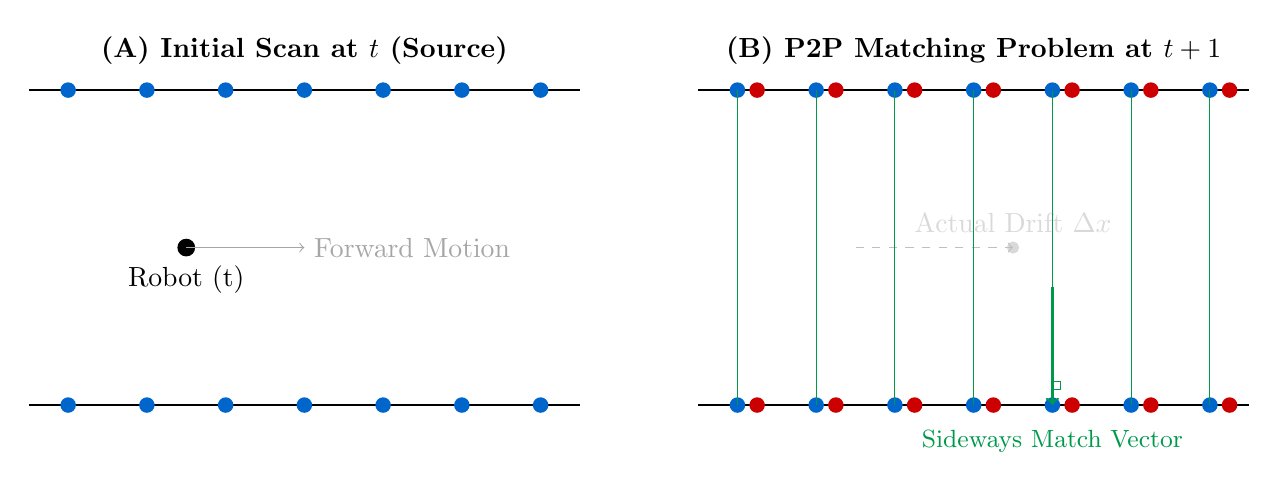
\begin{tikzpicture}[scale=1.0]

    % ==========================================
    % --- Figure (A) ---
    % ==========================================
    \begin{scope}[shift={(0,0)}]
        % Draw featureless corridor walls
        \draw[thick, black] (-2, 2) -- (5, 2);   
        \draw[thick, black] (-2, -2) -- (5, -2); 

        % Label
        \node[anchor=south] at (1.5, 2.2) {\textbf{(A) Initial Scan at $t$ (Source)}};

        % Generate source points
        \foreach \x in {-1.5, -0.5, 0.5, 1.5, 2.5, 3.5, 4.5} {
            \fill[sourcecolor] (\x, 2) circle (2.8pt);   
            \fill[sourcecolor] (\x, -2) circle (2.8pt);  
        }

        % Robot reference and motion label
        \filldraw[black] (0,0) circle (3pt) node[anchor=north, yshift=-3pt] {Robot (t)};
        \draw[->, gray!70, thin] (0,0) -- (1.5,0) node[anchor=west] {Forward Motion};
    \end{scope}

    % ==========================================
    % --- Figure (B) ---
    % Shifted 8.5 units to the right to sit side-by-side
    % ==========================================
    \begin{scope}[shift={(8.5,0)}]
        % Draw identical walls
        \draw[thick, black] (-2, 2) -- (5, 2);
        \draw[thick, black] (-2, -2) -- (5, -2);

        % Label
        \node[anchor=south] at (1.5, 2.2) {\textbf{(B) P2P Matching Problem at $t+1$}};

        % Visualization of actual motion
        \filldraw[gray!30] (2, 0) circle (2pt) node[anchor=south, yshift=2pt] {Actual Drift $\Delta x$};
        \draw[->, gray!50, dashed] (0,0) -- (2,0);

        % Loop to draw points and sideways match vectors
        \foreach \x in {-1.5, -0.5, 0.5, 1.5, 2.5, 3.5, 4.5} {
            % Source points (Blue)
            \fill[sourcecolor] (\x, 2) circle (2.8pt);
            \fill[sourcecolor] (\x, -2) circle (2.8pt);
            
            % Target points (Red, shifted forward by 2.0)
            \fill[targetcolor] ({\x + 0.25}, 2) circle (2.8pt); 
            \fill[targetcolor] ({\x + 0.25}, -2) circle (2.8pt); 
            
            % Sideways P2P vectors (Green)
            \draw[matchcolor, thin] (\x, 2) -- (\x, -2); 
        }
        
        % Example label for orthogonality
        \draw[matchcolor, ->, thick] (2.5, -0.5) -- (2.5, -2);
        \node[anchor=north, matchcolor, font=\small] at (2.5, -2.2) {Sideways Match Vector};
        \draw[matchcolor, thin] (2.5, -1.8) -- (2.6, -1.8) -- (2.6, -1.7) -- (2.5, -1.7) -- cycle; % Orthogonality symbol
    \end{scope}

\end{tikzpicture}

\end{document}